\section{Aplicações}
\label{s.application}

\begin{frame}{Aplicações}
	\begin{itemize}
		\justifying
		\item Modelagem de Linguagem com Máscaras;
		\\~\\
		\item Modelagem de Linguagem Causal;	
		\\~\\
		\item \emph{Bot} para Augmentação de Dados.
	\end{itemize}
\end{frame}

\begin{frame}{Modelagem de Linguagem com Máscaras}
	\begin{figure}[!ht]
		\centering
		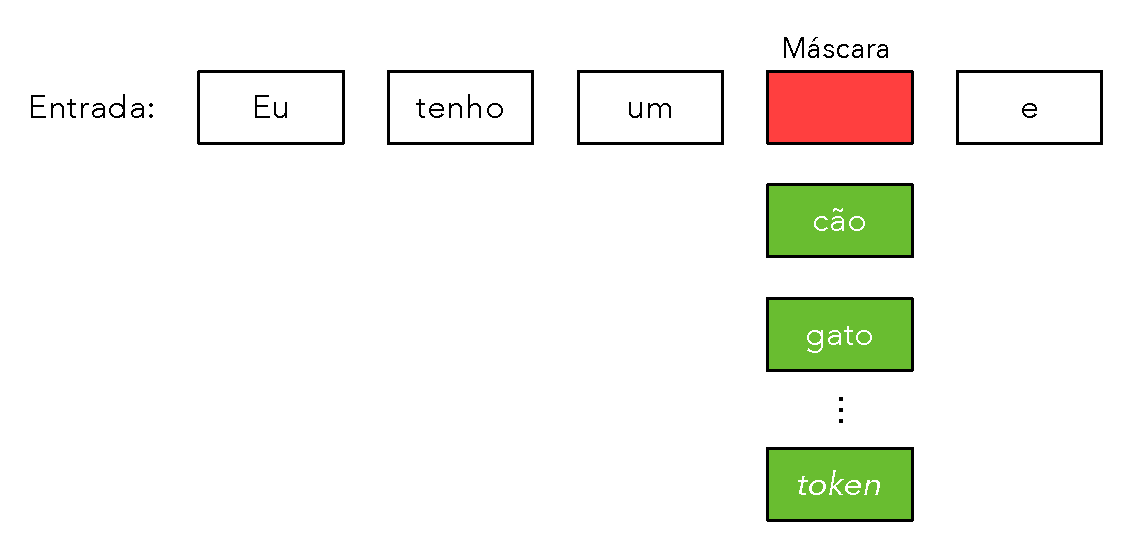
\includegraphics[scale=0.45]{figs/masked_lm.eps}	
		\label{f.masked_lm}
		\caption{Processo de modelagem de linguagem com máscaras.}
	\end{figure}
	Código: \url{https://github.com/gugarosa/text_augmenter/tree/master/applications/masked}
\end{frame}

\begin{frame}{Modelagem de Linguagem Causal}	
	\begin{figure}[!ht]
		\centering
		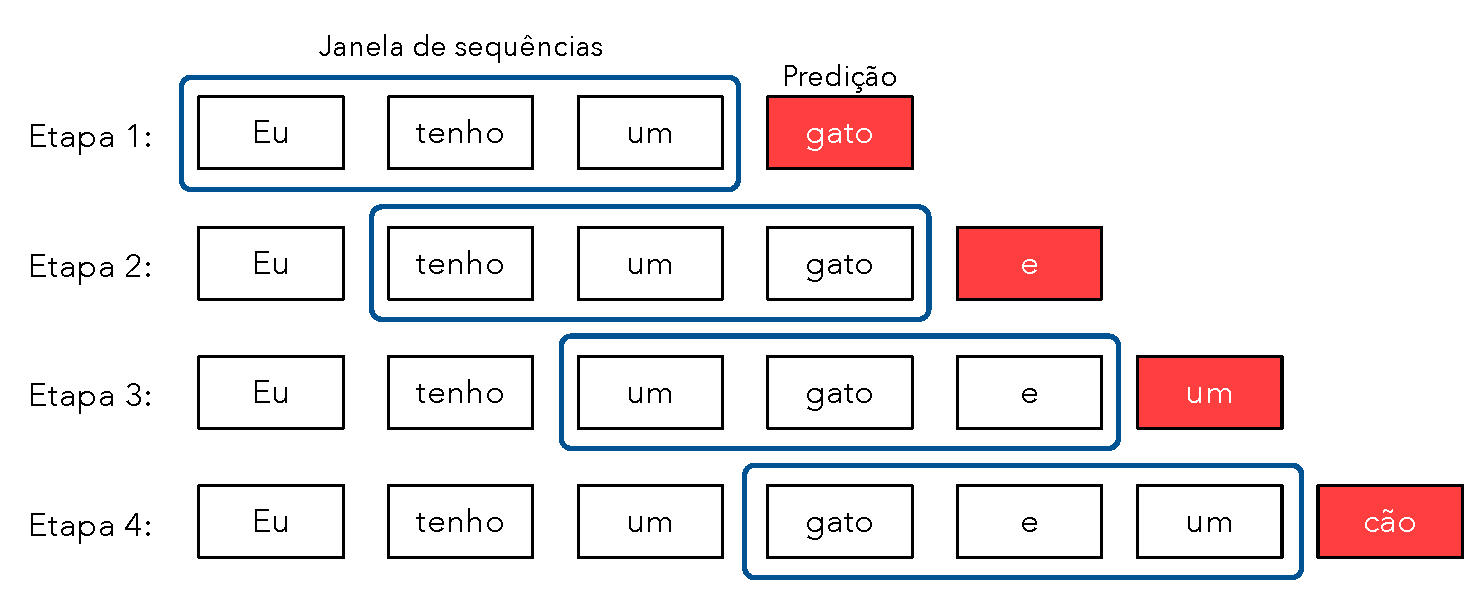
\includegraphics[scale=0.425]{figs/text_generation.eps}	
		\label{f.causal_lm}
		\caption{Processo de modelagem de linguagem causal.}
	\end{figure}
	Código: \url{https://github.com/gugarosa/text_augmenter/tree/master/applications/causal}
\end{frame}

\begin{frame}{\emph{Bot} para Augmentação de Dados}
	\begin{figure}[!ht]
		\centering
		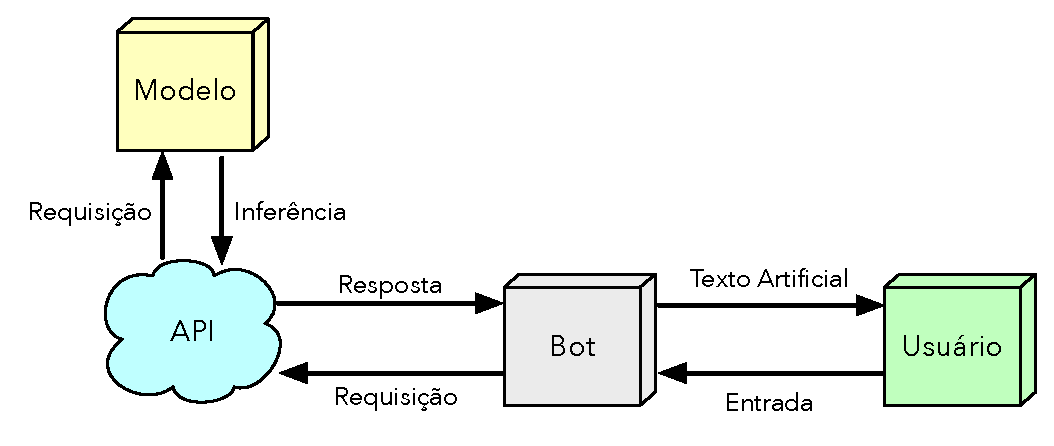
\includegraphics[scale=0.45]{figs/bot.eps}	
		\label{f.bot}
		\caption{Fluxograma de um \emph{bot} para augmentação de dados.}
	\end{figure}
	Código: \url{https://github.com/gugarosa/text_augmenter/tree/master/applications/bot}
	\\~\\
	Telegram: @RecognaBot
\end{frame}
